\section{Resultate und Vergleich}
In diesem Abschnitt geht es nun um die eriehlten Resultate und
einem Vergleich zwischen der rekursiven und iterativen
Implementation. Um einen solchen Vergleich zu ermöglichen habe
ich folgende Funktionen zum Berechnen der Laufzeit implementiert.
Die Perioden definieren wieviel mal die Finonacci-Zahl
berechnet wird und daraus wird dann der Mittelwert genommen.
So werden stark abweichende Messungen verhindert:

\begin{mdframed}[backgroundcolor=bg]
    \inputminted{Python}{src/time_fibonacci.py}
\end{mdframed}

\newpage

Um einen einfacheren Vergleich zu ermöglichen habe ich
für die definition der Tests die matplotlib verwendet.
Diese ermöglicht es einfach aus Zahlen ein visuelles
Diagramm zu erstellen. Die Implementation des Vergleichs
sieht folgendermassen aus:

\begin{mdframed}[backgroundcolor=bg]
    \inputminted{Python}{src/time_fibonacci_test.py}
\end{mdframed}

Wie nachfolgende ganz deutlich aus den Diagrammen herauszulesen ist,
ist die iterative Implementation definitiv mit Abstand performanter.
Bei der 3000. Fibonacci-Zahl ergibt sich eine 5x bessere
Performance. Und würde dann noch die Caching Funktionalität
der optimierten Version zum tragen kommen, wäre der
Performancegewinn noch einmal deutlich grösser.

\begin{figure}[h]
    \centering
    \caption{Die rekursive Implementation}
    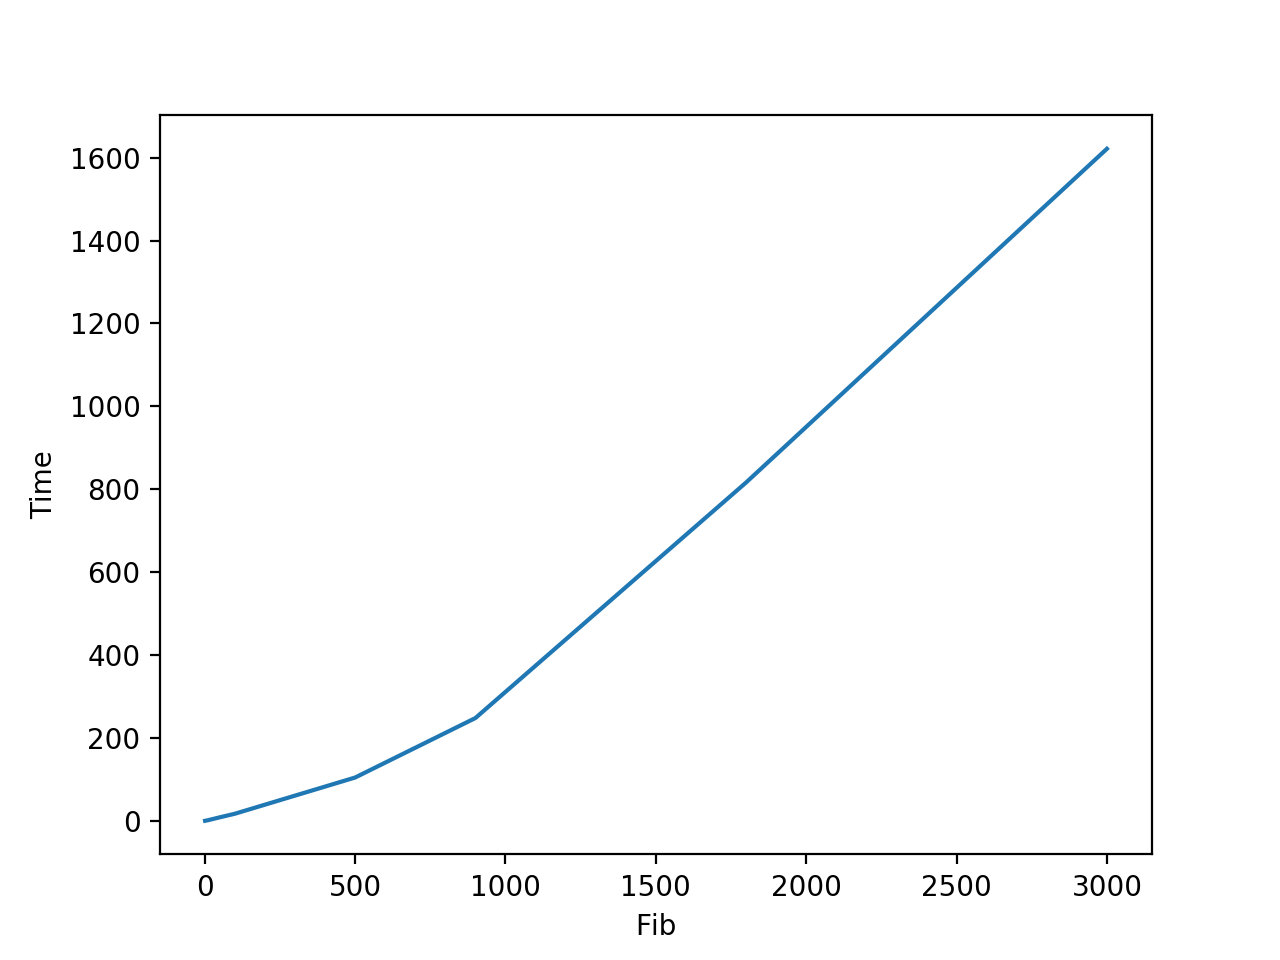
\includegraphics[width=0.8\textwidth]{Figure_1}
    \caption{Die iterative Implementation}   
    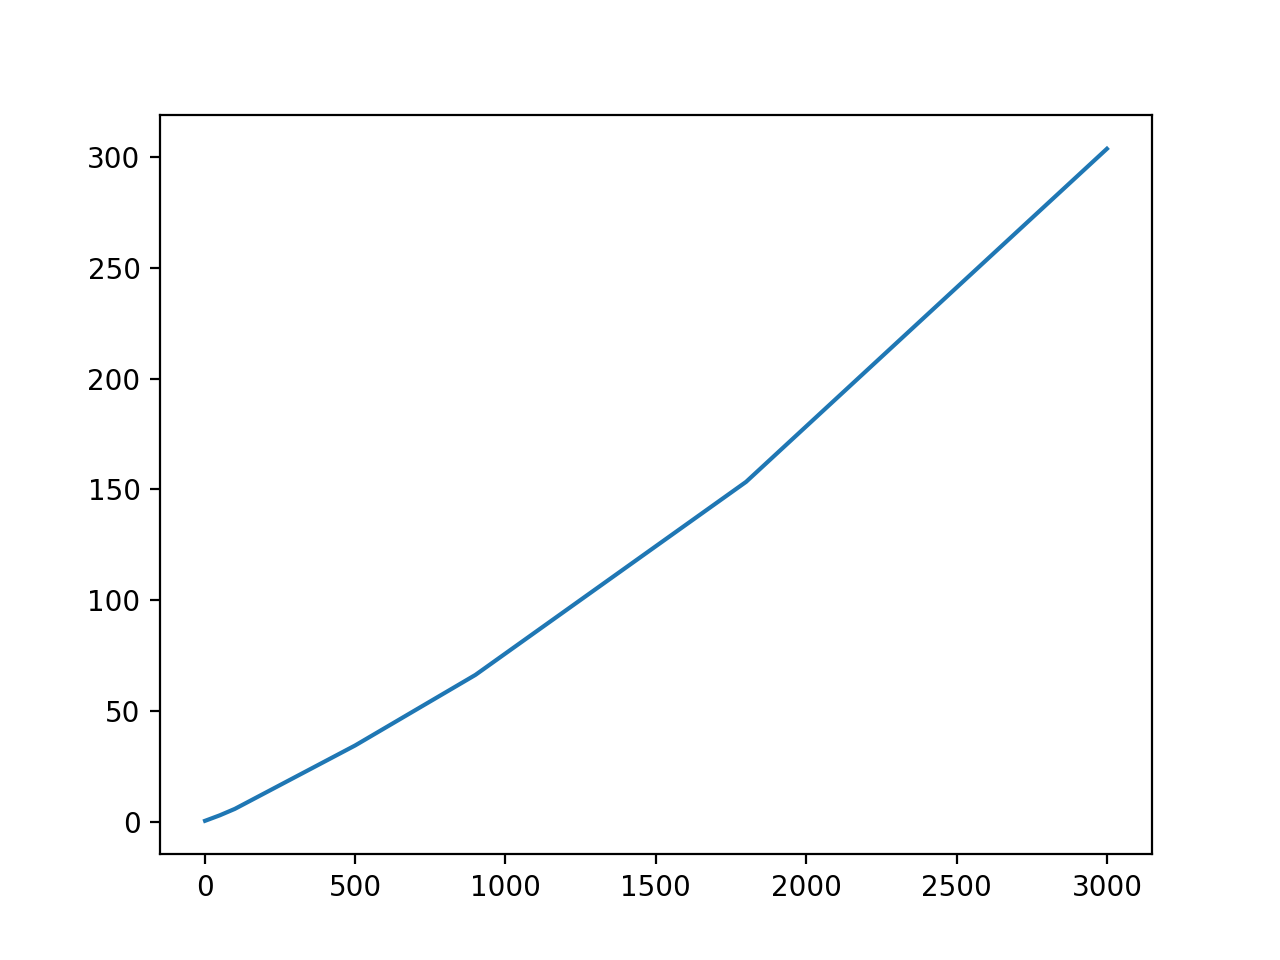
\includegraphics[width=0.8\textwidth]{Figure_2}
\end{figure}